\chapter{Data Fusion and State Estimation}
This chapter is dedicated to explaining the mathematical methods and models used to fuse data generated by the cameras and smartphone. It details the design and implementation of an EKF using MATLAB software. Kim et al. \cite{kim2011kalman} and source code provided by Patel served as the foundation of this chapter. All files pertaining to the filter have been included on the accompanying CD.

A good starting point for this chapter would be to define the states of interest of our system. We choose our states to be various parameters relating to the human gait and the bodies pose and position in the inertial frame. The model used in this work has various constants (the lengths of the rigid beams making up the limbs), but many changing parameters (the angles these rigid beams make with each other). These angles quantify the position of the various joints during steady state running and have therefore been chosen as states.

We cannot directly measure these angles since we have no sensors directly connected to them. All the system states are predicted by the EKF using various measurements relating directly and indirectly to them. The following table specifies the parameters used to symbolize the states of the system.
   
\begin{table}[!ht]
\centering
\label{statesForEkf}
\begin{tabular}{ll}
State & Description \\
$x_{body}$  	&x Position of body w.r.t. the inertial frame\\
$y_{body}$     &y Position of body w.r.t. the inertial frame\\
$z_{body}$     &z Position of body w.r.t. the inertial frame\\
$\phi_{body}$      &Roll of body w.r.t. the inertial frame\\
$\theta_{body}$    &Pitch of body w.r.t. the inertial frame\\
$\psi_{body}$      &Yaw of body w.r.t. the inertial frame\\
$\theta_{LH}$     &Pitch of left thigh w.r.t. left hip\\
$\psi_{LH}$      &Yaw of left thigh w.r.t. left hip\\
$\theta_{LK}$    &Pitch of left calf w.r.t. left knee\\
$\theta_{LA}$   &Pitch of left foot w.r.t. left ankle\\
$\theta_{RH}$    &Pitch of right thigh w.r.t. right hip\\
$\psi_{RH}$      &Yaw of right thigh w.r.t. right hip\\
$\theta_{RK}$   &Pitch of the right calf w.r.t. right knee\\
$\theta_{RA}$  &Pitch of the right foot w.r.t. the right ankle\\
\end{tabular}
\caption{Table showing the different states of the model to be determined by the EKF}
\end{table}

\newpage
Our system is not only concerned with these positional and angular elements, but also how they change over time. These rates where defined as the derivative of the states with respect to time. The first derivative serving as velocity and angular velocity, while the second derivative serves as acceleration and angular acceleration. Here the vector \textbf{x} serves as a element of our state vector \textbf{X}.

$$\textbf{x} = [ x_{body} \; y_{body} \; z_{body} \; \phi_{body} \;    		    \theta_{body}  \; \psi_{body}\;  \theta_{LH}\; \psi_{LH}   \;\theta_{LK} 	\;\theta_{LA} 	\;\theta_{RH} \;\psi_{RH}   	\;\theta_{RK}   \; \theta_{RA}  		]$$ 

$$	\textbf{X}=[\textbf{x} \; \dot{\textbf{x}} \; \ddot{\textbf{x}}] $$

The vector \textbf{x} contains 14 elements. From the above equations it is clear that our state vector \textbf{X} contains 42 elements. With the states of our system defined we must discuss state estimation and the critical elements of the EKF.

\section{State Estimation}
The key purpose of the Kalman Filter is the ability to estimate the various states of our system. To understand how this estimation will occur we need to firstly understand the KF. The following diagram shows the critical parts of the KF.

\begin{figure}[!ht] 
\captionsetup{width=0.8\linewidth, font=small}  
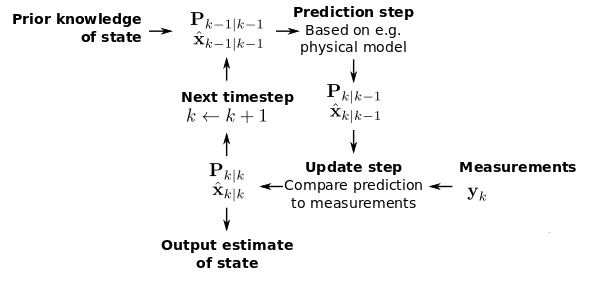
\includegraphics[width=0.6\linewidth]{figures/kf.png}
\caption{Figure showing the interplay of various elements of the KF, adapted from \cite{kfkfkf}}
\label{fig:kf}
\end{figure}

The critical elements of the KF as seen in the diagram are: the states themselves, a prediction model, an update model, measurements, initialization values, and various uncertainty models. 

The underlying equation of the KF is the \textit{process equations}, where the state value at the next time instance $ X_{k+1} $ is predicted by applying the transition matrix $ F_{k+1} $ to the state values at the current time instance $ X_{k} $ and adding a zero mean Gaussian noise term $ w_{k} $. The $ w $ element of this equation is collected in the process noise matrix $ Q $. 

$$ X_{k+1} = F_{k+1}X_{k} + w_{k}  $$

Another underlying equation of the KF is the \textit{measurement equation}. Here the observable measurements contained in $ Y_k $ are related to the states at the current time instance $ X_{k} $ through the measurement matrix $ H_{k} $. A zero mean Gaussian noise term $ v_{k} $ is added to account for measurement uncertainty. The various measurement uncertainties are collected in the measurements noise matrix $ R $. 

$$ Y_k = H_{k}X_{k} + v_{k} $$


As discussed in the literature review, the KF can only be applied to linear systems. The EKF is the extension of the filter so that it may be applied to nonlinear systems. To introduce the workings of the EKF we start by defining a classic nonlinear system defined by the state space model

$$ X_{k+1} = f(k,X_{k}) + w_{k}  $$

$$ Y_k = h(k,X_{k}) + v_{k} $$

In this representation $ w_{k} $ and $ v_{k} $ are consistent with definitions given for the KF and are contained in matrices $ Q $ and $ R $ respectively. From the state space equations one can see that we now predict states using a nonlinear transition matrix function $ f $ and $ h $.

These functions can be defined by their anti-derivative matrices $F$ and $H$ respectively.

$$ F_{k+1,k} = \frac{\delta f(k,X_{k})}{\delta x} $$

$$ H_{k} = \frac{\delta h(k,X_{k})}{\delta x} $$

These are the fundamental equations of the KF and EKF. We can now 

\section{Process Equations}
The fundamental assumption made when deriving the prediction equations for our states was that the acceleration (both linear and angular) was constant between sampling intervals. It would therefore stand that the positional states of the filter $[x_{body} \; y_{body} \; z_{body}]$ and the angular states of the filter $[\theta_{body} \; ... \; \theta_{RA}]$ could be predicted using: 

$$ \ddot{p}_{k+1} = \ddot{p}_{k} + \sigma_{\ddot{p}}^{2} $$
$$ \dot{p}_{k+1} = \dot{p}_{k} + \ddot{p}_{k}T + \sigma_{\dot{p}}^{2} $$
$$ p_{k+1} = p_{k} + \dot{p}_{k}T + \sigma_{p}^{2} $$

for the positional states, and:

$$ \ddot{\alpha}_{k+1} = \ddot{\alpha}_{k} + \sigma_{\ddot{\alpha}}^{2} $$
$$ \dot{\alpha}_{k+1} = \dot{\alpha}_{k} + \ddot{\alpha}_{k}T + \sigma_{\dot{\alpha}}^{2} $$
$$ \alpha_{k+1} = \alpha_{k} + \dot{\alpha}_{k}T + \sigma_{\alpha}^{2} $$

for the angular states.

These prediction equations where created in MATLAB using symbolic functions. The sigma associated each equations takes into account the prediction uncertainties contained in the Q matrix. By adjusting these values we can increase the filter performance. This is discussed further in a later section.

\section{Measurement Equations}
The measurement equations for the lower limbs where generated using inverse kinematics. This requires a model

\subsection{Euler Matrices}
The following matrices are the rotational matrices for rotating a point in 3D space along a certain axis. 

$$
Roll(\phi) = 
\begin{bmatrix} 
1 & 0 & 0 \\ 
0 & \cos{\phi} & -\sin{\phi} \\ 
0 & \sin{\phi} & \cos{\phi}  
\end{bmatrix}
$$


$$
Pitch(\theta) = 
\begin{bmatrix} 
\cos{\theta} & 0 & \sin{\theta} \\ 
0 & 1 & 0 \\ 
-\sin{\theta} & 0 & \cos{\theta}  
\end{bmatrix}
$$


$$
Yaw(\psi) = 
\begin{bmatrix} 
\cos{\psi} & -\sin{\psi} & 0 \\ 
\sin{\psi} & \cos{\psi} & 0 \\ 
0 & 0 & 1  
\end{bmatrix}
$$


\subsection{Direct Cosine Matrix}


\subsection{Forward Kinematics}

\textbf{front}\\
right knee
$$ p1xyz = bodyY + bodyZ + R1 * Thigh $$
left knee
$$ p2xyz = bodyY + bodyZ + R1 * Thigh $$
right foot
$$ p3xyz = bodyY + bodyZ + R1 * Thigh + R2 * Calf + R3 * Foot $$
left foot
$$ p4xyz = bodyY + bodyZ + R1 * Thigh + R2 * Calf + R3 * Foot $$

\textbf{back}\\
right calf
$$ p1xyz = bodyY + bodyZ + R1 * Thigh + R2 * 0.5 * Calf $$
left calf
$$ p2xyz = bodyY + bodyZ + R1 * Thigh + R2 * 0.5 * Calf $$
right heel
$$ p2xyz = bodyY + bodyZ + R1 * Thigh + R2 * Calf $$
left heel
$$ p2xyz = bodyY + bodyZ + R1 * Thigh + R2 * Calf $$

\section{Camera Matrix}

It is important to understand the different parameters that mathematically quantify cameras. These parameters can be devided into \textit{extrinsic} and \textit{extrinsic}. Extrinsic camera variables related to the cameras position in the inertial frame and the direction the camera is facing. These can be summarized by the extrinsic camera matrix 

$$[ R \, |\, \boldsymbol{t}] = 
\left[ \begin{array}{ccc|c} 
r_{1,1} & r_{1,2} & r_{1,3} & t_1 \\
r_{2,1} & r_{2,2} & r_{2,3} & t_2 \\
r_{3,1} & r_{3,2} & r_{3,3} & t_3 \\
\end{array} \right]$$


\section{Q Matrix, R Matrix and Initialization}
This section will discuss the final components of the EKF namely the Q matrix containing the various process noise variations, R matrix containing the various measurement noise variances and the initial state values.

\subsection{Defining the Q Matrix}
From the above equations we can see that the Q matrix must have dimensions of $n*n$, where $n$ in this equation is the total amount of states. As previously defined in this section our filter operates over 42 states, giving Q a size of $42*42$. All the variance parameters will be contained on the diagonal of the matrix with all other entries being zero.

To find the initial values of these uncertainties the derivative of the various accelerations where taken. The maximum element from that set was selected as the uncertainty parameter.

\subsection{Defining the R Matrix}
The R matrix relates to the measurement variables and must therefore have size of $m*m$, where $m$ is the amount of inputs the EKF. These are elements of the sensors themselves and can be found by researching the relative data sheets for the smartphone IMU. As for the cameras a relatively large uncertainty of about 5 pixels was assumed.

\subsection{Choosing Initial States}
The subject was stationary during the initial stages of the run. This allows us to initialize our state vector with all states initially zero. The filter will therefore track the transience and steady state estimation of a running subject, giving insight into the filters performance under different conditions. 


\subsection{Initializing the Covariance Matrix P}
following on from the previous section zeroing the initial states of the system allows us to have a relatively small initial covariance matrix due to the relative certainty we have that the states are truly zero. 


 








